\documentclass{beamer}

\usepackage[backend=biber,style=ieee]{biblatex} % Load biblatex package
\addbibresource{../paper/bibliography.bib}
%\usepackage{natbib}


% Set the theme to a simple, clean style
\usetheme{default}
\usecolortheme{default}
\setbeamertemplate{itemize item}{\normalsize\textbullet} % Change bullets to dots
\setbeamertemplate{footline}[frame number]

\usepackage{graphicx}
\usepackage{amsmath}
\usepackage{algorithm}
\usepackage{algpseudocode}
\usepackage{pythontex}
\usepackage{float}
\usepackage{booktabs}


\title{Variational Oblique Predictive Clustering Trees}
\author{Viktor Andonovikj}
\institute{Jožef Stefan Institute \& Jožef Stefan International Postgraduate School}
\date{\today}

\begin{document}

\setbeamertemplate{section in toc}[ball unnumbered]

% Title slide
\begin{frame}[plain]
  \titlepage
\end{frame}

% Outline slide
\begin{frame}[plain]
  \frametitle{Outline}

  {\small % Reduce font size
    \setlength{\baselineskip}{10pt} % Adjust line spacing
    \tableofcontents
  }

\end{frame}


\addtocounter{framenumber}{-2}

\section{Key Idea}
\begin{frame}
  \frametitle{Key Idea}
  \begin{itemize}
    \item We focus on \textbf{decision tree} type of models - popular due to their interpretability and simplicity.
    \item We aim to combine the \textbf{predictive power} of \textbf{ensemble} methods with the \textbf{interpretability} of a \textbf{single} decision tree.
    \item \textbf{Variational SPYCT} incorporates Bayesian inference to enhance both predictive performance and decision-making transparency.
  \end{itemize}
\end{frame}


\section{Introduction to Structured Output Prediction}
\begin{frame}
  \frametitle{Introduction to Structured Output Prediction (SOP)}
  \begin{itemize}
    \item \textbf{Structured Output Prediction (SOP)} involves predicting multiple interdependent outputs.
    \item SOP tasks include simultaneous prediction of:
      \begin{itemize}
        \item Multiple continuous values.
        \item Multiple discrete values.
        \item Hierarchically organized discrete values.
      \end{itemize}
    \item \textbf{Real-world applications}:
      \begin{itemize}
        \item Drug discovery: predicting multiple biological properties of molecules.
        \item Recommender systems: predicting user preferences across multiple items.
        \item Genomics: predicting gene functions based on interdependent traits.
      \end{itemize}
  \end{itemize}
\end{frame}


\begin{frame}
  \frametitle{Predictive Clustering Framework}
  \begin{itemize}
    \item \textbf{Predictive Clustering}: Combines clustering and prediction by treating prediction as a hierarchical clustering task where similar instances are grouped and predictions are made for each cluster.
    \item \textbf{Characteristics}:
      \begin{itemize}
        \item Supports both supervised and semi-supervised learning.
        \item State-of-the-art performance via ensemble learning.
        \item Offers interpretable models through feature importance analysis.
        \item Provides a unified framework for predictive modeling across multiple tasks.
      \end{itemize}
  \end{itemize}
\end{frame}


\begin{frame}
  \frametitle{Predictive Clustering Trees (PCT) vs Oblique Predictive Clustering Trees (SPYCT)}
  
  \begin{figure}
    \centering
    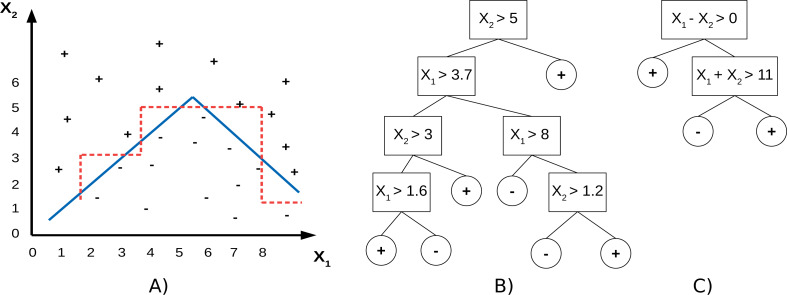
\includegraphics[width=0.75\textwidth]{images/pct_spyct.jpg}
    {\tiny \caption{A) Learned split - SPYCT in blue, PCT in red B) PCT C) SPYCT~\cite{Stepi_nik_2021}}}
  \end{figure}
  
  \vspace{0.05cm} % Reduces space between the image and text
  
  \begin{itemize}
    \item \textbf{PCT}: Uses axis-aligned splits (based on single features), fully interpretable models.
    \item \textbf{SPYCT}: Uses oblique splits (linear combinations of features), more flexibility for high-dimensional and sparse data, suited for more complex tasks with intricate decision boundaries.
  \end{itemize}
  
\end{frame}


\begin{frame}
\frametitle{Introduction to Variational SPYCT}
  \begin{figure}
    \centering
    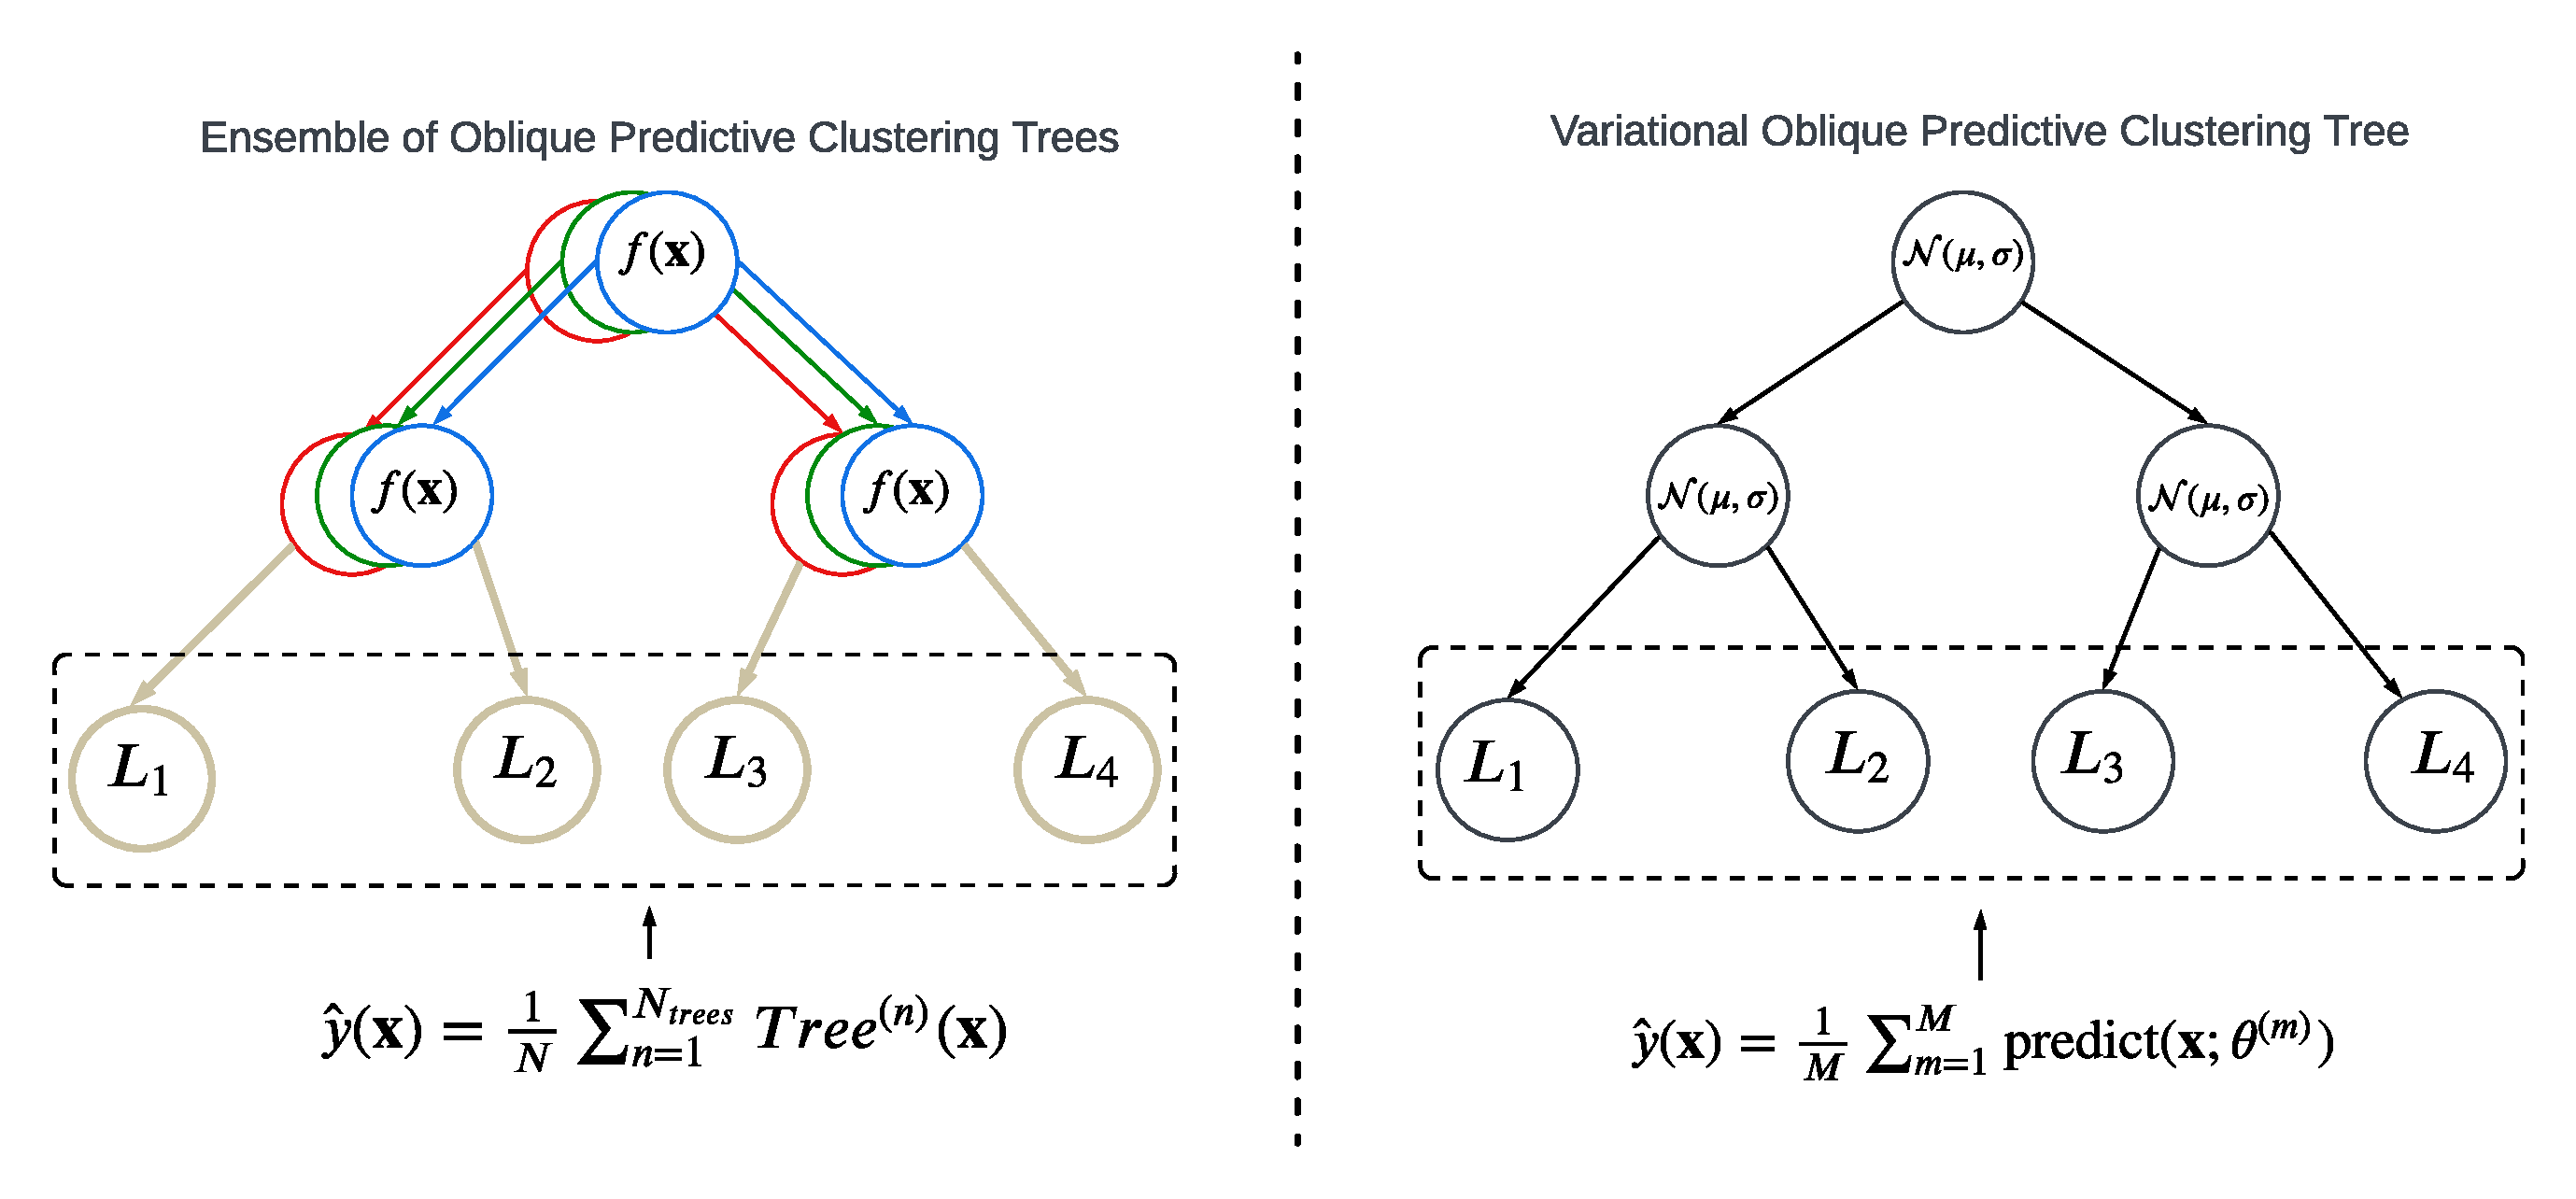
\includegraphics[width=1.0\textwidth]{../figures/main_flowchart.pdf}
    {\tiny \caption{Ensemble of SPYCTs vs Variational SPYCT}}
  \end{figure}
\end{frame}

\section{Variational SPYCT}
\begin{frame}
  \frametitle{Introduction to Variational SPYCT}
  \begin{itemize}
    \item \textbf{Motivation}: Variational SPYCT (VSPYCT) integrates variational Bayes for improved decision-making within a single model, eliminating the need for ensembles.
    \item \textbf{Uncertainty quantification}: Embeds Bayesian inference directly into the decision tree structure, providing insight into decision processes and confidence levels.
    \item \textbf{Novelty}: VSPYCT introduces probabilistic treatment of oblique splits, offering a paradigm shift toward interpretable, and reliable machine learning models.
  \end{itemize}
  
\end{frame}


\begin{frame}
  \frametitle{Optimization through Variational Bayes}
  
  \small % Reduce text size to fit within margins
  
  \begin{itemize}
    \item \textbf{Bayes' Theorem}: 
      \[
      p(\theta|x) = \frac{p(x|\theta) p(\theta)}{p(x)}
      \]
    \item The primary computational challenge lies in calculating the posterior $p(\theta|x)$, where the denominator $p(x)$ requires:
      \[
      p(x) = \int_{\theta} p(x|\theta) p(\theta) \,d\theta
      \]
    \item \textbf{Variational Bayes (VB)} approximates the posterior with $q_{\omega^*}(\theta)$, minimizing the KL divergence:
      \[
      \omega^* = \arg\min_{\omega \in \Omega} KL(q_\omega(\theta) \parallel p(\theta|x))
      \]
    \item The Evidence Lower Bound (ELBO) is maximized to improve the approximation:
      \[
      KL(q_\omega(\theta) \parallel p(\theta|x)) = - \mathbb{E}_q[\log p(x,\theta) - \log q_\omega(\theta)] + \log p(x)
      \]
    \item VB's computational efficiency surpasses methods like MCMC, though it introduces bias based on the choice of the variational family $\mathcal{Q}$.
  \end{itemize}
  
\end{frame}

\begin{frame}
\frametitle{Optimization through Variational Bayes}
  \begin{figure}
    \centering
    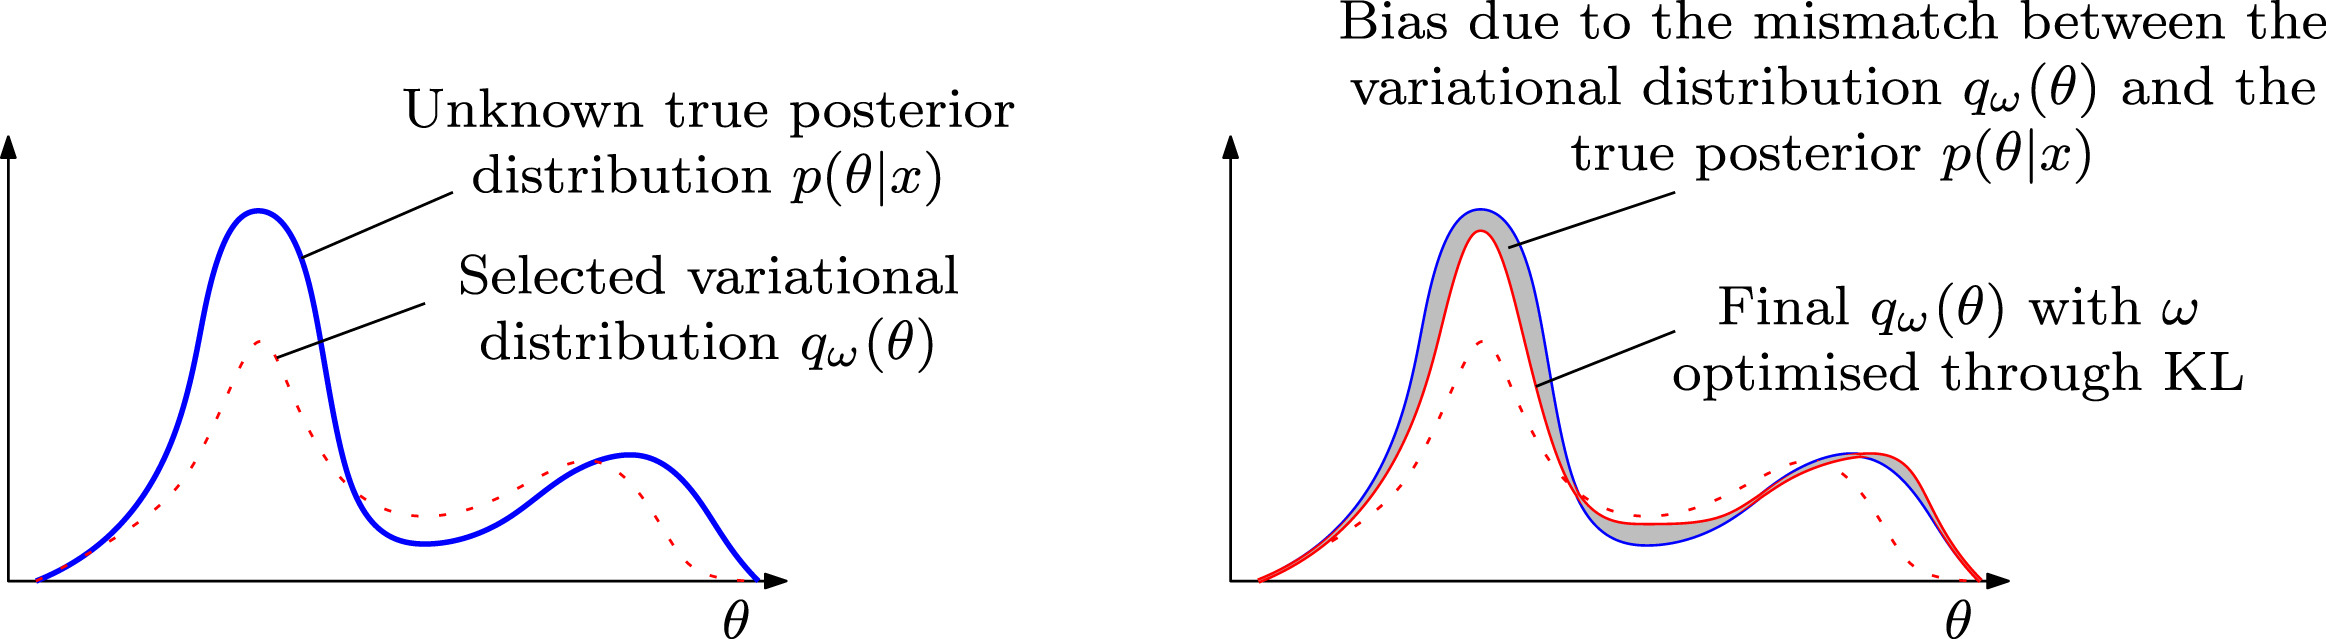
\includegraphics[width=1.0\textwidth]{images/vb_optim.jpg}
    {\tiny \caption{Optimisation process of finding the closest variational distribution $q_\omega(\theta)$ over the set of latent variables $\omega$.~\cite{}}}
    \end{figure}
\end{frame}

\begin{frame}
  \frametitle{Methodology Overview}
  \begin{itemize}
    \item VSPYCT follows SPYCT's tree-based architecture, but replaces fixed parameters with random variables.
    \item \textbf{Key difference}: VSPYCT uses variational Bayes (VB) for probabilistic split optimization, improving handling of noisy data and uncertainty.
    \item Split parameters (weights $\mathbf{w}$ and bias $b$) are modeled as random variables, allowing uncertainty estimation.
  \end{itemize}
  \[
  f(\mathbf{x}) = \sigma \left(\mathbf{w}^\top \mathbf{x} + b \right)
  \]
\end{frame}

\begin{frame}
  \frametitle{Learning Splits through Variational Bayes}
  \begin{itemize}
    \item Weights $\mathbf{w}$ and bias $b$ have Gaussian priors:
    \[
    \mathbf{w} \sim \mathcal{N}(\mathbf{0}, \mathbf{I}), \quad b \sim \mathcal{N}(0, 1)
    \]
    \item Variational Bayes approximates the posterior distribution with:
    \[
    q(\mathbf{w}, b|\mathcal{D}) = \mathcal{N}(\mathbf{w}|\boldsymbol{\mu}_w, \boldsymbol{\Sigma}_w) \mathcal{N}(b|\mu_b, \sigma_b^2)
    \]
    \item ELBO maximization: 
    \[
    \mathcal{L}(\boldsymbol{\mu}, \boldsymbol{\Sigma}) = \mathbb{E}_{q(\mathbf{w}, b|\mathcal{D})}[\log p(\mathcal{D}|\mathbf{w}, b)] - KL(q(\mathbf{w}, b|\mathcal{D}) \parallel p(\mathbf{w}, b))
    \]
  \end{itemize}
\end{frame}

\begin{frame}
  \frametitle{Algorithm for Learning a Split}
  
  \centering
  \begin{algorithm}[H]
  \caption{Variational Learning of Split Parameters}
  \label{alg:learn_split_vb}
  \begin{algorithmic}[1]
      \State \textbf{Input:} $\mathcal{D} = \{\mathbf{X}, \mathbf{Y}\}$, $\theta = \{\mathbf{w}_0, b_0\}$, $E$ (epochs), $\lambda$ (learning rate), $\beta$ (batch size), $\sigma$ (selection probability)
      \State \textbf{Output:} $\Theta = \{\boldsymbol{\mu}_w, \boldsymbol{\Sigma}_w, \mu_b, \sigma_b^2\}$ (variational parameters)
   
      \Procedure{LearnSplit}{$\mathcal{D}, \theta, E, \lambda, \beta, \sigma$}
          \State Initialize $\Theta = \{\boldsymbol{\mu}_w, \boldsymbol{\Sigma}_w, \mu_b, \sigma_b^2\}$
          \For{$e \in \{1, \dots, E\}$}
              \For{each mini-batch $\mathcal{B} \subseteq \mathcal{D}$ of size $\beta$}
                  \State Sample $\mathbf{w} \sim \mathcal{N}(\boldsymbol{\mu}_w, \boldsymbol{\Sigma}_w)$, $b \sim \mathcal{N}(\mu_b, \sigma_b^2)$
                  \State Compute impurity $\Omega(\mathbf{X}, \mathbf{Y}; \mathbf{w}, b)$
                  \State Compute ELBO $\mathcal{L}(\mathcal{B}; \Theta)$
                  \State Update $\Theta$
              \EndFor
          \EndFor
          \State \textbf{return} $\Theta$
      \EndProcedure
  \end{algorithmic}
  \end{algorithm}
\end{frame}


\begin{frame}
  \frametitle{Deriving the Impurity Function}

  \begin{itemize}
    \item For a given split node \(i\), we define the fuzzy membership:
    \[
    FM_i = \sigma(\mathbf{x}^\top \mathbf{w_i} + b_i), \quad 1 - FM_i = \text{right group membership}
    \]

    \item The split fitness function is the following:
    \[
    f(\mathbf{w_i}, b_i) = Z \cdot imp(FM) + (L + U - Z) \cdot imp(1 - FM)
    \]
    \item Impurity is given by the variances of the target \(Y\) and features \(X\):
    \[
    imp(FM) = \sum_{k=1}^{N} \sigma_{\bar{X}_k}^2 + \sum_{k=1}^{T} \sigma_{\bar{Y}_k}^2
    \]
  \end{itemize}

  \begin{itemize}
    \item In VSPYCT, we minimize this impurity by observing a target impurity of $impurity/2$ at each step using Variational Bayes.
  \end{itemize}

\end{frame}



\begin{frame}
  \frametitle{Making a Prediction}
  \begin{itemize}
    \item Prediction involves traversing the tree, making probabilistic decisions at each node.
    \item The split is determined by evaluating the function:
 \[
  f(\mathbf{x}) = \sigma \left(\mathbf{w}^\top \mathbf{x} + b \right)
  \]
    \item The final prediction $\hat{y}$ is the prototype value at the reached leaf:
    \[
    \hat{y} = \frac{1}{|\mathbf{Y}|} \sum_{i=1}^{|\mathbf{Y}|} y_i
    \]
  \end{itemize}
\end{frame}


\begin{frame}
  \frametitle{Prediction Process in VSPYCT}

  \footnotesize
  \setlength{\intextsep}{1pt}
  \setlength{\textfloatsep}{1pt}

  \begin{algorithm}[H]
    \caption{Prediction using Monte Carlo Sampling}
    \label{alg:make_pred}
    \begin{algorithmic}[1]
      \State \textbf{Input:} Feature vector $\mathbf{x}$, tree $T$, samples $M$
      \State \textbf{Output:} Prediction $\hat{y}$
      
      \State Initialize $\hat{y}_{\text{sum}} = 0$
      \For{$m = 1$ to $M$}
        \State Traverse $T$ from root to leaf with sampled $\mathbf{w}^{(m)}, b^{(m)}$
        \State $\hat{y}_{\text{sum}} \gets \hat{y}_{\text{sum}} + $ prediction at leaf
      \EndFor
      \State \Return $\hat{y} = \frac{\hat{y}_{\text{sum}}}{M}$
    \end{algorithmic}
  \end{algorithm}
  
\end{frame}


\begin{frame}
  \frametitle{Feature Importance}
  \begin{itemize}
    \item Feature importance in VSPYCT: Calculated as the influence of features across all splits.
    \item The importance of a feature is determined by:
    \[
    \text{Imp}(T) = \sum_{s \in T} \left( \frac{s_n}{N} \right) \left( \frac{\mathbb{E}[\mathbf{w}_s]}{|\mathbb{E}[\mathbf{w}_s]|_1} \right)
    \]
    \item Weights $\mathbf{w}$ are sampled from the posterior distribution, and importance is aggregated over all splits.
  \end{itemize}
\end{frame}



\begin{frame}
  \frametitle{Time Complexity Analysis}
  \begin{itemize}
    \item Time complexity of learning a split in VSPYCT:
    \[
    \mathcal{O}(MNI_{vb}(D+K))
    \]
    \item $M$: Number of Monte Carlo samples, $N$: Data points, $D$: Features, $K$: Clustering attributes, $I_{VB}$: Number of optimization iterations.
  \end{itemize}
\end{frame}

\section{Experimental Setting}
\begin{frame}
  \frametitle{Experimental Setting}
  \begin{itemize}
    \item \textbf{Comparison}: VSPYCT vs SPYCT (single tree and ensemble).
    \item \textbf{Tasks}: Single-target and multi-target regression, binary and multi-class classification.
    \item \textbf{Goal}: Evaluate predictive performance of VSPYCT across different modeling scenarios.
  \end{itemize}
\end{frame}

\section{Data}
\begin{frame}
  \frametitle{Data}
  \begin{itemize}
    \item Datasets cover regression and classification tasks.
    \item Number of examples (N), features (D), targets (T), and classes (C).
  \end{itemize}
  
  \begin{table}[h!]
    \centering
    \caption{Summary of the datasets used in the experiments.}
    \label{tab:datasets}
    \scriptsize % Reduce font size to fit the table
    \begin{tabular}{lcccccc}
    \toprule
    \textbf{Dataset} & \textbf{Type of Task} & \textbf{N} & \textbf{D} & \textbf{T} & \textbf{C} \\
    \midrule
    rf1~\cite{mulan}              & Multi-target regression  & 9125   & 64   & 8  & -- \\
    rf2~\cite{mulan}              & Multi-target regression  & 9125   & 576  & 8  & -- \\
    atp1d~\cite{mulan}            & Multi-target regression  & 337    & 411  & 6  & -- \\
    atp7d~\cite{mulan}            & Multi-target regression  & 296    & 411  & 6  & -- \\
    scm1d~\cite{mulan}            & Multi-target regression  & 9803   & 280  & 16 & -- \\
    house\_8L~\cite{openml}        & Single-target regression & 22784  & 8    & 1  & -- \\
    puma8NH~\cite{openml}          & Single-target regression & 8192   & 8    & 1  & -- \\
    diabetes~\cite{openml}         & Binary classification    & 768    & 8    & 1  & 2 \\
    banknote~\cite{openml}         & Binary classification    & 1372   & 4    & 1  & 2 \\
    gas-drift~\cite{openml}        & Multi-class classification & 13910 & 128  & 1  & 6 \\
    balance~\cite{openml}          & Multi-class classification & 625   & 4    & 1  & 3 \\
    \bottomrule
    \end{tabular}
  \end{table}
  
\end{frame}

\begin{frame}
  \frametitle{Evaluation Metrics}
  \begin{itemize}
    \item \textbf{Regression}: Mean Absolute Error (MAE).
    \[
    \textit{MAE} = \frac{1}{N} \sum_{i=1}^{N} \left| y_i - \hat{y}_i \right|
    \]
    \item \textbf{Classification}: F1 score (macro-averaged for multi-class tasks).
    \item \textbf{Cross-validation}: 5-fold cross-validation used to reduce bias.
  \end{itemize}
\end{frame}

\section{Results}
\begin{frame}
  \frametitle{Regression Results}

  \begin{table}[h!]
    \centering
    \caption{\textit{MAE} Scores for Regression Datasets}
    \label{tab:regression_results}
    \scriptsize
    \begin{tabular}{lccc}
    \toprule
    \textbf{Dataset} & \textbf{SPYCT-single tree} & \textbf{SPYCT-ensemble} & \textbf{VSPYCT} \\
    \midrule
    rf1            & 29.38         & \textbf{29.34}  & 29.37 \\
    rf2             & 29.37         & 29.49           & \textbf{29.36} \\
    atp1d           & 95.17         & \textbf{70.93}  & 77.24 \\
    atp7d           & 115.54        & \textbf{73.08}  & 91.28 \\
    scm1d           & 205.99        & 206.01          & \textbf{205.72} \\
    house\_8L       & 25378.02      & \textbf{19817.56} & 22992.24 \\
    puma8NH         & 2.80          & \textbf{2.62}   & 2.74 \\
    \bottomrule
    \end{tabular}
  \end{table}

  \vspace{0.2cm}
  \begin{itemize}
    \item VSPYCT outperforms or closely matches the SPYCT ensemble on several datasets (rf2, scm1d).
    \item Ensemble methods generally achieve lower MAE, but VSPYCT provides competitive results.
  \end{itemize}
  
\end{frame}


\begin{frame}
  \frametitle{Classification Results}
  
  \begin{table}[h!]
    \centering
    \caption{F1 Scores for Classification Datasets}
    \label{tab:classification_results}
    \scriptsize
    \begin{tabular}{lccc}
    \toprule
    \textbf{Dataset} & \textbf{SPYCT-single tree} & \textbf{SPYCT-ensemble} & \textbf{VSPYCT} \\
    \midrule
    diabetes              & 0.53                            & \textbf{0.60}            & 0.59 \\
    banknote              & 0.97                            & \textbf{0.99}            & 0.98 \\
    gas-drift             & 0.98                            & 0.99            & \textbf{0.99} \\
    balance               & 0.60                            & 0.66                     & \textbf{0.73} \\
    \bottomrule
    \end{tabular}
  \end{table}
  
  \vspace{0.2cm}
  \begin{itemize}
    \item VSPYCT achieves competitive performance across datasets, often matching or surpassing ensembles.
    \item In the balance dataset, VSPYCT achieves the best F1 score.
  \end{itemize}
  
\end{frame}

\section{Interpretability}
\begin{frame}
  \frametitle{Interpretability - An example with real dataset}

  \begin{itemize}
    \item \textbf{Dataset:} Unemployment dataset from the Slovenian Public Employment Service (PES), consisting of 74,086 anonymized instances.
    \item \textbf{Features:} Age, gender, education, work experience, and other personal/professional characteristics.
    \item \textbf{Target:} Time until the jobseeker becomes employed or exits the study (measured in days). Some records are right-censored (event not observed).
    \item \textbf{Goal:} Predict the time-to-event (employment) with censored data, using a semi-supervised learning approach for handling the inherent missing information.
    \item \textbf{Challenges:} Diverse attribute types (categorical, numerical, temporal) and the presence of censored data.
  \end{itemize}

\end{frame}

\begin{frame}
  \frametitle{Structure of the learned VSPYCT model}
  \begin{figure}
    \centering
    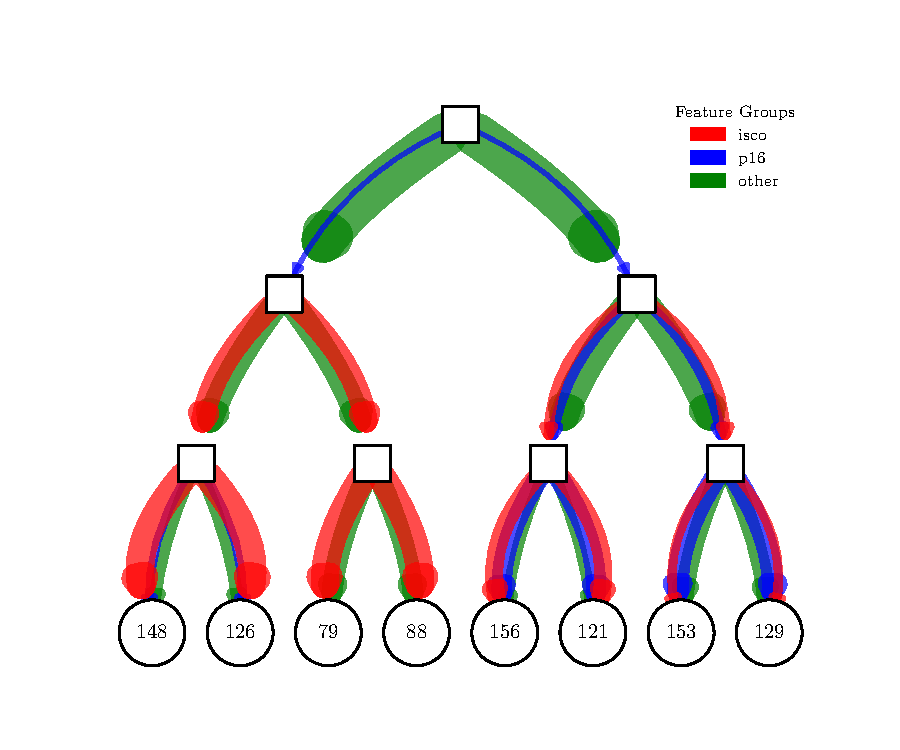
\includegraphics[width=0.8\textwidth]{../figures/hecat_tree_old_temp.pdf}
    \caption{VSPYCT tree structure. Colors represent different feature groups (e.g., education, profession).}
  \end{figure}
\end{frame}


\begin{frame}
  \frametitle{Predicted Survival Curve}
  \begin{figure}
    \centering
    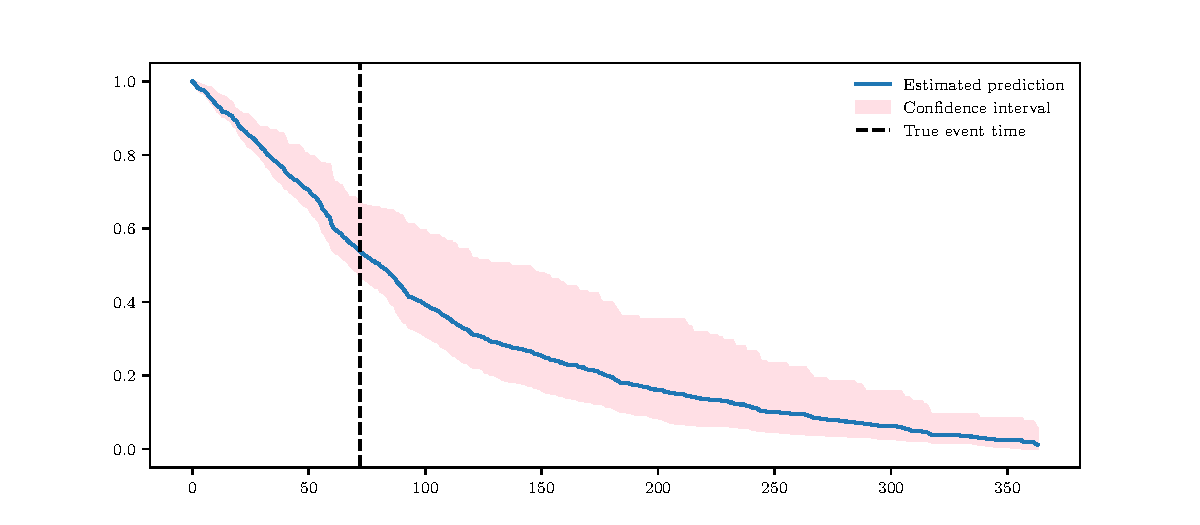
\includegraphics[width=0.8\textwidth]{../figures//pred_with_ci.pdf}
    \caption{Predicted survival curve for a jobseeker. Blue: mean prediction; shaded area: confidence interval; vertical line: true event time.}
  \end{figure}
  \begin{itemize}
    \item The confidence interval captures the uncertainty behind the predictions.
  \end{itemize}
\end{frame}

\begin{frame}
  \frametitle{Feature Importance}
  \begin{figure}
    \centering
    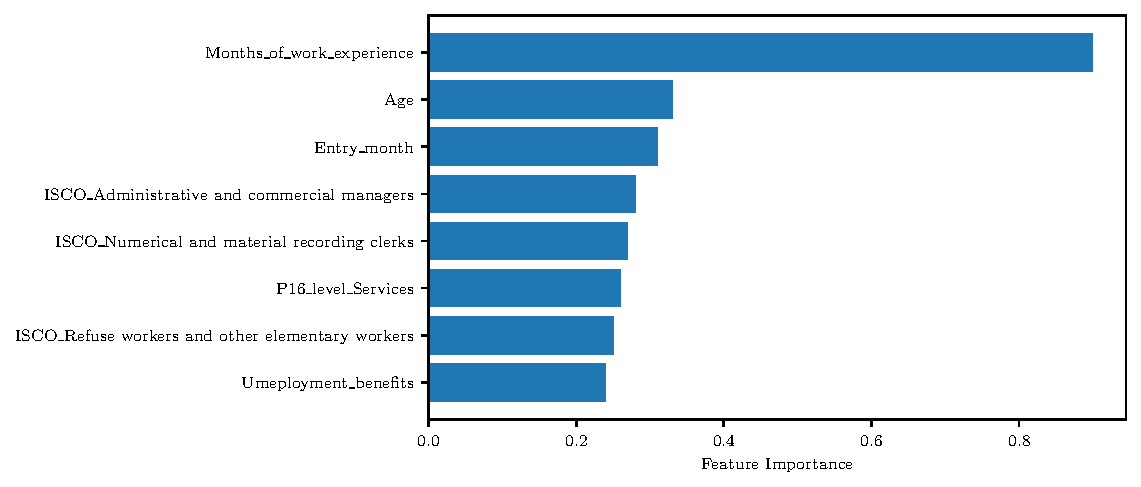
\includegraphics[width=0.8\textwidth]{../figures/feature_importance.pdf}
    \caption{Feature importance from the VSPYCT model. "Months of work experience" is the most important factor in the model's decisions.}
  \end{figure}
\end{frame}

\section{Conclusion}
\begin{frame}
  \frametitle{Conclusion}

  \begin{itemize}
    \item \textbf{VSPYCT Model:} Combines oblique splits, variational Bayes, and Bayesian inference in an interpretable predictive framework.
    \item \textbf{Key Characteristic:} Balances the performance of ensemble models with the interpretability of single decision trees, while introducing uncertainty quantification.
    \item \textbf{Results:} Competitive performance, sometimes surpassing ensembles of SPYCT.
    \item \textbf{Uncertainty Quantification:} Enhances decision-making reliability, making the model applicable to domains where certainty in predictions is critical.
    \item \textbf{Future Work:} Further performance improvements and extending applications to diverse predictive tasks.
  \end{itemize}

\end{frame}

\addtocounter{framenumber}{-2}

% Bibliography slide
\begin{frame}[allowframebreaks, plain] % Allows the bibliography to continue on multiple slides if necessary
  \frametitle{References}
  \printbibliography
\end{frame}

% Thank You Slide
\begin{frame}[plain]
  \frametitle{Thank You}
  \centering
  Questions?
\end{frame}


\end{document}

